%%%%%%%%%%%%%%%%%%%%%%%%%%%%%%%%%%%%%%%%%%%%%%%%%%%%%%%%%%%%%%%%%%%%%%%%%%%%%%%%
%2345678901234567890123456789012345678901234567890123456789012345678901234567890
%        1         2         3         4         5         6         7         8

\documentclass[letterpaper, 10 pt, conference]{ieeeconf}  % Comment this line out
                                                          % if you need a4paper
%\documentclass[a4paper, 10pt, conference]{ieeeconf}      % Use this line for a4
                                                          % paper

\IEEEoverridecommandlockouts                              % This command is only
                                                          % needed if you want to
                                                          % use the \thanks command
\overrideIEEEmargins
% See the \addtolength command later in the file to balance the column lengths
% on the last page of the document



% The following packages can be found on http:\\www.ctan.org
%\usepackage{graphics} % for pdf, bitmapped graphics files
%\usepackage{epsfig} % for postscript graphics files
%\usepackage{mathptmx} % assumes new font selection scheme installed
%\usepackage{times} % assumes new font selection scheme installed
%\usepackage{amsmath} % assumes amsmath package installed
%\usepackage{amssymb}  % assumes amsmath package installed
\usepackage{algorithmic}
\usepackage{amsmath}
\usepackage{array}
\usepackage{url}
\usepackage{svg}
\usepackage{amsfonts}
\usepackage{bm}
\usepackage{hyperref}
\usepackage{epigraph}
\usepackage{booktabs}
\usepackage{float}
\usepackage{multirow}
\usepackage{tikz}
\usepackage{graphicx}
\usepackage{caption}
\usepackage{cite}
\title{\LARGE \bf
A Comparative Study of Deep Learning Approaches in Off-Line Network Intrusion Detection
}

%\author{ \parbox{3 in}{\centering Huibert Kwakernaak*
%         \thanks{*Use the $\backslash$thanks command to put information here}\\
%         Faculty of Electrical Engineering, Mathematics and Computer Science\\
%         University of Twente\\
%         7500 AE Enschede, The Netherlands\\
%         {\tt\small h.kwakernaak@autsubmit.com}}
%         \hspace*{ 0.5 in}
%         \parbox{3 in}{ \centering Pradeep Misra**
%         \thanks{**The footnote marks may be inserted manually}\\
%        Department of Electrical Engineering \\
%         Wright State University\\
%         Dayton, OH 45435, USA\\
%         {\tt\small pmisra@cs.wright.edu}}
%}

\author{Jiaqi Yan$^{1}$ and Dong Jin$^{2}$% <-this % stops a space
%\thanks{*This work was not supported by any organization}% <-this % stops a space
\thanks{$^{1}$J. Yan is a PhD candidate of Computer Science,
        Illinois Institute of Technology, 10 West 35th Street, Chicago, IL 60616, USA
        {\tt\small jyan31 at hawk.iit.edu}}%
\thanks{$^{2}$D. Jin is an associate professor with the Department of Computer Science,
		Illinois Institute of Technology,
        10 West 35th Street, Chicago, IL 60616, USA
        {\tt\small dong.jin at iit.edu}}%
}


\begin{document}



\maketitle
\thispagestyle{empty}
\pagestyle{empty}


%%%%%%%%%%%%%%%%%%%%%%%%%%%%%%%%%%%%%%%%%%%%%%%%%%%%%%%%%%%%%%%%%%%%%%%%%%%%%%%%
\begin{abstract}
Network intrusion detection system (NIDS) is essential to the security of any communication systems.
Recently a handful of novel deep neural networks bundled with more advanced and smarter
training algorithms have achieved unprecedentedly good performance on image classification,
natural language processing, speech recognition and many other research branches.
Motivated by these impressive improvements in the field of artificial intelligence,
this paper introduces a bunch of deep learning models to the design of NIDS
and conducts a comparative evaluation of these models.
Firstly, we introduce general deep learning methodology and its potential implication on the
network intrusion detection problem.
Then we briefly review the existing machine learning solutions to two network intrusion detection tasks,
namely the NSL-KDD dataset and the UNSW-NB15 dataset.
After describing a set of cutting-edge deep learning models,
we conduct a quantitatively comparative evaluation of them with the help of
our own TensorFlow-based deep learning library, NetLeaner.
\end{abstract}

\section{Introduction}

Network intrusion detection system (NIDS) is the essential security technology that
aims to protect any networked systems efficiently and automatically.
As either a hardware device or software application,
it monitors a network for malicious activities or policy violations.
By intercepting and analyzing the bi-direction traffics through the network,
it raises alarm if intrusion, attack or violation are observed.
There are two general approaches to detect intrusions.
In signature based intrusion detection, e.g. SNORT~\cite{Snort},
rules for specific attacks are pre-installed in the system.
It report suspicious traffic when the traffic matches any signature of known attacks.
The major drawback of signature matching approach is that
it is only effective for previously detected attacks that have an identifiable signature.
As a result, signature database needs to be manually updated whenever a new type of attack
is discovered, with significant effort, by the network administrator.
Anomaly detection based approach overcomes these limitations by adopting a certain
type of machine learning technique to model the trustworthy network activities.
Traffics that significantly deviates from the built model are treated as malicious.
This idea have been shown to be able to detect unknown or novel attacks~\cite{NSL-KDD, STL-NIDS}.
However, if the built model for normal traffics are not generalized enough,
anomaly based approach will treat unforeseen normal traffic as malicious,
suffering from high false positive.

In this project, we follow the anomaly detection based idea, and tries to enhance it with the
state-of-art machine learning technology, e.g. various deep neural networks trained by innovative algorithms.
Specifically, we have made the following contributions:
\begin{itemize}
    \item Firstly, we introduce the background of deep learning models and techniques,
        and discuss why they may better solve the network intrusion detection problem.
    %Besides, we also survey and discuss the status quo of available network intrusion detection datasets
    %and its implication on applying deep learning models to network intrusion detection.
    \item Then we briefly review the existing state-of-the-art machine learning solutions to network intrusion detection.
        After that, we describe several groups of the cutting-edge deep learning models
        in concisely mathematical languages.
    \item We conduct a quantitatively comparative study of each of them with
        two off-line network intrusion detection datasets~\cite{NSL-KDD, UNSW},
        with the help of our own TensorFlow-based deep learning library, NetLeaner.
        The detection performance is measured in accuracy, precision and recall.
    \item We not only make the codebase of NetLearner publicly available to research community,
        but also share the deep learning related hacks and tricks used during the training phase,
        so that future researches can easily reproduce and extend our work.
\end{itemize}


\section{Deep Learning Background}
We introduce two main reasons behind the success of deep learning to the rise of artificial intelligence as well as the implications of deep learning for network intrusion detection.

In the supervised learning framework, given the feature representations and inference models, learning is an optimization process that minimizes a predefined loss function over the training examples.
The most commonly-used optimization algorithm is back-propagation (BP)~\cite{Backpropagation} with gradient descent,
because computing gradient is Hessian-free and memorization saves a significant amount of computation when propagating backward level by level.
However, it is challenging to train deep neural networks with optimal weights only using BP.
The first problem is that the cost function is usually non-convex, and
optimizing algorithms only with the first-order gradient is likely to be stuck at a poor local minimum.
Secondly, exploding and vanishing gradient makes back-propagation difficult to train models with many layers stacked together,
such as deep recurrent neural networks.
Even if we can tolerate the long training time and carefully deal with the gradient exploding and vanishing,
the trained model is often over-fitted to the training dataset, and thus fails to generalize to the testing or future datasets.

The emergence of many novel learning algorithms and training techniques enables us to train deep neural networks that achieve good suboptimal minimums.
For example, stochastic gradient descent (SGD) with mini-batches can significantly increase the training speed comparing
to normal gradient descent on the entire dataset.
In each step of gradient descent, researchers have shown that momentum can
prevent SGD from ``oscillating across but pushing along the shallow ravine"~\cite{Momentum}.
Along with decaying learning rate, momentum-based optimization algorithms (e.g., Adam~\cite{Adam}) often find better local minimums.
To prevent over-fitting, researchers have proposed dropout~\cite{Dropout} to average over an exponential number of neural networks.
These general learning algorithms and training techniques would directly help neural networks to achieve better performance for the network intrusion detection problem.

Another breakthrough in the deep learning area is that researchers have successfully trained a number of useful unsupervised generative models.
Different from supervised models or discriminative models that aim to discover the relationship between input variables and target labels (or the conditional probability distribution of the targets given the inputs),
these models aim to learn the joint probability distribution or the joint conditional distribution of all variables for one phenomenon from the given dataset.
The resulting generative model is powerful in many ways.
First, given the well-trained probability distribution, the model can synthesize meaningful data comparable to real examples in the training set.
For example, Auxiliary-Classifier Generative Adversarial Nets (AC-GAN)~\cite{AC-GAN} can generate high-quality images after training on ImageNet dataset~\cite{ImageNet};
both AC-GAN and deep brief nets~\cite{DeepBeliefNets} can synthesize handwritten digits after learning from the MNIST dataset.
Second, the ability to generate high quality faked data indicates that
the model has learned better feature representations from the unlabeled data.
For example, the features extracted from the hidden units of sparse autoencoder can significantly improve the performance of support vector classifier~\cite{SparseAE}.
Additionally, researchers have shown that it is an excellent strategy to initialize deep neural networks with the weights from a successfully trained generative model~\cite{DeepBeliefNets, Momentum}.

In the area of network intrusion detection, the amount of network traffic data is massive,
%e.g., in the order of terabytes per day in a large monitored network. In practice, the amount of data is 
which makes it hard for security analysts to find malicious patterns and label anomalies.
This situation makes the unsupervised generative model a promising solution
to traffic classification. %since it can be trained unsupervised:
First, it utilizes the vast amount of unlabeled data to learning useful and hierarchical features. Second, it effectively initializes the weights of the hidden layers in a deep neural network, which allows further fine-tuning towards a high-performance classifier.
Among the various deep learning models we investigate in this paper, there are two types of generative models, i.e., restricted Boltzmann machine and autoencoders.

%In addition to the sophisticated and efficient learning algorithms, abundant open data in the domain of image classification, natural language processing, or machine translation actually drive the novel and complex neural network models and make them successful.
%Table~\ref{Tab:Datasets} lists the dimension and amount of the training dataset for various image classification tasks.

\iffalse
The most vivid example would be how ImageNet dataset~\cite{ImageNet} pushed a series of deep learning models,
such as AlexNet, GoolgNet and ResNet, who greatly improved the performance of visual object recognition.
ImageNet organizes a large amount of web images by synonym set, multiple words or word phrases
describing a meaningful concept.
On average each synonym set is illustrated by 1000 quality-controlled and human-annotated images.
This project was first presented at 2009 Conference on Computer Vision and Pattern Recognition by researchers
from the CS department at Princeton University, and ran as an annual software contest known as
ImageNet Large Scale Visual Recognition Challenge (ILSVRC) since 2010.
The state-of-the-art error rate of this competition was near 25\%,
until in the year of 2012, a deep convolutional neural networks AlexNet~\cite{AlexNet} trained on GPU achieved a winning top-5 error rate of 15.3\%.
From then on, deep neural networks with convolutional blocks start its showtime.
GooLeNet~\cite{GoogLeNet} won the ILSVRC 2014 with top-5 error rate of 6.7\%.
It has 22 layers and strayed from the simple design of stacking convolutional and pooling layers.
One year later, residual block based ResNet~\cite{ResNet} pushed the error rate further down to 3.6\% with even deeper architecture.
\fi

%\begin{table*}[]
%\centering
%\caption{Popular Datasets used in Deep Learning v.s. Available Network Traffic Datasets}
%\label{Tab:Datasets}
%\begin{tabular}{c|c|c|c|c}
%\multicolumn{1}{c|}{Domain}                          & Dataset Name  & \#Examples in Training Set & Feature Dimension            & Instance-Feature Ratio \\
%\hline
%\hline
%\multirow{6}{*}{Image}                               & MNIST         & 60,000        & 784 (28$\times$28 gray images)            & 76.53    \\
                                                     %& SVHN          & 600,000       & 3072 (32$\times$32 color images)          & 195.31   \\
                                                     %& CIFAR-10      & 60,000        & 3072 (32$\times$32 color images)          & 19.53    \\
                                                     %& Tiny          & 80 million    & 3072 (32$\times$32 color image            & 26041.67 \\
                                                     %& ImageNet      & 1.2 million   & 196,608 (256$\times$256 color images)     & 18.31   \\
%\hline
%\multicolumn{1}{l|}{\multirow{2}{*}{Network Traffic}} & UNSW-NB15    & 175,341       & 42                                        & 4174.79 \\
%\multicolumn{1}{l|}{}                                 & NSL-KDD      & 125,973       & 41                                        & 3072.51
%\end{tabular}
%\end{table*}

\section{Existing Works}
Due to the large number of network intrusion detection systems that adopt machine learning or data mining approaches
we only review a few of them that achieve state-of-the-art detection performance.
There are very limited number of existing network intrusion detection systems that adopt
deep learning approaches.
Their details can be found in section~\ref{Sec:Architectures}.

\subsection{State-of-Art Machine Learning Approaches}
Prior researchers modeled the intrusion detection task as an unsupervised
anomaly detection problem, and proposed a series of approaches.
Examples include Mahalanobis-distance based outliner detection~\cite{ComparativeAnomalyNIDS},
density-based outliner detection~\cite{LOF, ComparativeAnomalyNIDS},
evidence accumulation for ranking outliner~\cite{RankingOutliner}, etc.
One of the advantage of these unsupervised approaches is to tackle the problem of
the unavailability of labeled traffic data.

Alternatively, prior researchers made a lot of effort to obtain meaningful
attacking data and to convert them into labeled data~\cite{DARPA, KDDCup, NSL-KDD, UNSW, UNSW1}.
Such efforts make it possible to apply supervised machine learning algorithms to the
intrusion detection problem.
Successfully applied approaches include decision trees~\cite{DecisionTree},
linear and non-linear support vector machines~\cite{SVM}, NB-Tree~\cite{NB-Tree} and so on.
To the best of the authors' knowledge, there are two works that achieved the best prediction
accuracy on the two different datasets respectively.
For the UNSW-NB15 dataset, it is reported in~\cite{RampLossKSVCR} that extending K-support vector
classification-regression~\cite{KSVCR} with ramp loss, called Ramp-KSVCR approach, can achieve the state-of-the-art accuracy of 93.52\%.
The authors of Ramp-KSVCR also report that their approach can achieve 98.68\% accuracy on the NSL-KDD dataset.
On the other hand, the creators of UNSW-NB15 dataset~\cite{UNSW} proposed an approach called
Geometric Area Analysis techniques using trapezoidal area estimation (GAA-ADS for short)~\cite{GAA-ADS}.
It achieves the bese known accuracy on NSL-KDD dataset (99.7\%) and a slightly worse accuracy on
UNSW-NB15 dataset (92.8\%).


\subsection{Deep Learning Flavor Approaches}
There are some pioneer works that introduced deep learning approaches to intrusion detection.
For example, \cite{STL-NIDS} adopts sparse autoencoder and the self-taught learning
scheme~\cite{SparseAE} to handle the problem of limited amount of labeled data for training supervised model.
Similar semi-supervised approach have also been applied to
Discriminative restricted Boltzmann machine~\cite{AnomalyDetectionRBM}.

\section{Offline Network Intrusion Detection Tasks}
Unlike image classification or natural language processing,
the labeled datasets in network intrusion detection tasks~\cite{KDDCup, DARPA, UNSW1, UNSW, NSL-KDD} lacks a common feature space.
For example, among the two most completed datasets NSL-KDD\cite{NSL-KDD} and UNSW-NB15~\cite{UNSW},
there are only three easy-to-identify common features: src\_bytes, dst\_bytes and service.
As a result, we consider each dataset are an standalone network intrusion detection task.
Among alternative available datasets,
we choose both NSL-KDD dataset and UNSW-NB15 dataset as our targeted tasks.
We list the dimension and amount of the NIDS training datasets that we used in this paper along with those famous image classification datasets in Table~\ref{Tab:Datasets}.

\subsection{NSL-KDD Dataset}
The NSL-KDD dataset originates from the KDDCup 99 dataset~\cite{KDDCup},
which was used for the third International Knowledge Discovery and Data Mining Tool Competition.
NSL-KDD dataset addresses two issues of the KDDCup 99 dataset.
First, it eliminates the redundant records in the KDDCup 99 that take up
78\% and 75\% of the records in train and test set, respectively.
Second, it samples the dataset such that the fraction of the record from a difficulty level
is inversely proportional to its difficulty.
Both enhancements make NSL-KDD dataset more suitable for
evaluating intrusion detection systems.

The train dataset consists of 125,973 TCP connection records, while the test dataset
consists of 22,544 ones.
A record is defined by 41 features, including 9 basic features of individual
TCP connections, 13 content features within a connection and 9 temporal features computed
within a two-second time window, and 10 other features.
Connections in the train dataset are labeled as either normal or one of the 24 attack
types.
There are additional 14 types of attacks in the test dataset, intentionally designed to
test the classifier's ability to handle novel attacks.
The task of the classifier is to identify whether a connection is normal or one of the
4 categories of attacks, namely denial of service (DoS), remote to local (R2L), user to
root (U2R) and probing, also known as 5-class classification problem.

\subsection{UNSW-NB15 Dataset}
Similar to KDDCup 99 dataset, the UNSW-NB15 dataset is generated by simulating normal
and attack behaviors in a hardware testbed.
The simulation is conducted in the Cyber Range Lab of the Australian Centre for Cyber Security (ACCS)
and 49 features in the dataset is extracted by a chain of software tools also developed by ACCS.
The structure of the features is similar to that of KDDCup 99: 5 flow features,
13 basic features, 8 content features, 9 time features and 12 other features.
However, there are only a couple of common features to the NSL-KDD dataset.
The size of the dataset is 257,673 in term of flow records, 175,341 of which are used for
training set and the rest are for testing.
There are nine types of attacks in the dataset.
The only common type of attack between UNSW-NB15 and NSL-KDD is DoS.
The new attacks in UNSW-NB15 are analysis, backdoor, exploits, fuzzers, generic, reconnaissance, shellcode, and worms.
In this project, we consider the 2-class classification problem for UNSW-NB15 dataset: the
task of the classifiers is to predict a given traffic is either normal or malicious.

\section{Deep Learning Architectures}
\label{Sec:Architectures}

In this section, we introduce a bunch of deep learning models that we consider promising in the
network intrusion detection problem.
For each architecture, we first give a brief mathematical introduction of it.
Then we describe how we build and train the model using a Python library NetLearner~\cite{NetLearner}.
NetLearner implements these deep learning models on the basis of TensorFlow.\footnote{TensorFlow~\cite{TensorFlow} is an open-source software library for machine learning developed by the Google Brain Team.}

\subsection{Multilayer Perceptron}
\label{SubSec:MLP}
Multilayer perceptron (MLP) is a classic deep learning classifier with simple
design of the connectivity between neurons.
It is a fully connected feed-forward neural network, as shown in Figure~\ref{Fig:MLPArchitecture}.
By introducing non-linear neural units (perceptrons), it can distinguish data that are
not linearly separable.
However, the non-linearity make it very hard to train a deep MLP of more than three layers,
even if people have proposed the efficient back-propagation learning algorithm~\cite{Backpropagation}.
Recently it revived due to the various new training techniques designed by deep learning community,
including Stochastic Gradient Descent (SGD), Adam optimizer~\cite{Adam},
batch normalization~\cite{BatchNorm} and Dropout~\cite{Dropout}.
Except for the number of neurons in each layer and number of layers,
MPL can also be tuned with different activation functions, or neural types.
The most popular two, which are used in this project, are logistic function
and rectifier linear unit.
Logistic function is written as
\begin{align}
    f(x) &= \frac{1}{1 + e^{-x}}
\end{align}
It has a very useful property when we applying back-propagation:
\begin{align}
    f'(x) &= f(x) (1-f(x))
\end{align}
Recently, most deep neural networks adopt rectifier neural unit and
achieved very good performance~\cite{DeepLearning}.
Rectifier linear unit is defined as
\begin{align}
    f(x) &= \max(0, x)
\end{align}
Let $\mathbf{a}^{(l)}$ be the activation of layer $l$,
$\mathbf{W}^{(l)}$ and $\mathbf{b}^{(l)}$ be layer $l$'s parameter.
With activation function defined, we have the following recursive formula that describes
the feed-forward step of the perceptron network.
\begin{align}
    \mathbf{z}^{(l+1)} &= \mathbf{W}^{(l)} \mathbf{a}^{(l)} + \mathbf{b}^{(l)} \label{Equ:MLPFeedForward1}\\
    \mathbf{a}^{(l+1)} &= f(\mathbf{z}^{(l+1)})
    \label{Equ:MLPFeedForward2}
\end{align}

\begin{figure}[h]
    \centering
    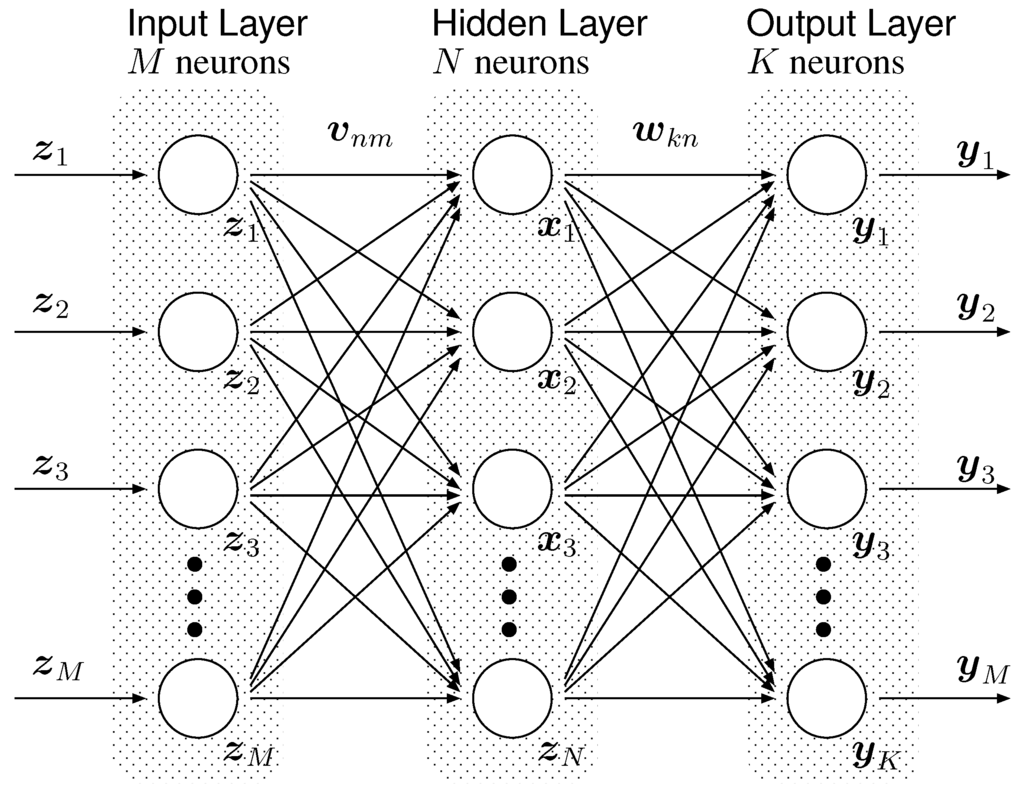
\includegraphics[width=0.45\textwidth]{figures/multilayer_perceptron.png}
    \caption{A multilayer perceptron neural network with 1 hidden layer.
        Figure courtesy of Teijiro Isokawa, Haruhiko Nishimura and Nobuyuki Matsui.}
    \label{Fig:MLPArchitecture}
\end{figure}

We build two dual-hidden-layer MLP, with 800 neurons in first layer,
and 480 neurons in the second layer followed by a softmax classifier,
one for the NSL-KDD task and the other for the UNSW-NB15 task.
Both MLP are trained with Adam optimizer~\cite{Adam} for 200 epochs and batch size 80.
During the training, learning rate decays from 0.1 exponentially with the base of 0.96.
We do not include regularization in the model, but do apply dropout of probability 0.2.
We denote both MLP models as MLP and show their detailed results in the later section.

\subsection{Restricted Boltzmann Machine}
Restricted Boltzmann machine (RBM)~\cite{RBMTechReport} is a type of energy-based model,
which associate a scalar energy to each configuration vector of the variables in the network.
In energy-based model, learning is the process of configuring the network weights so that
the average energy over training data is minimized.
RBM consists of a layer of hidden units (H) and a layer of visible units (V).
Here ``restricted" means that connections are just between hidden and visible layer,
but not within hidden layers or visible layers.
This makes its training to be faster than Boltzmann machine and makes it feasible to
stack multiple separately trained RBM together to form deep architecture.
A joint configuration, $(\mathbf{v, h})$, of the visible and hidden units has the energy of
\begin{align}
    E(\mathbf{v, h}) &= -\sum_{i\in visible}a_i v_i - \sum_{j\in hidden}b_j h_j - \sum_{i, j}v_i h_j w_{ij}
\end{align}
where $a=\{a_i\}$ and $b=\{b_j\}$ are biases in visible and hidden layer respectively,
and $W=\{w_{ij}\}$ is the weights between them.
The network assigns a probability to every possible pair of $(\mathbf{v, h})$ via this energy
function
\begin{align}
    p(\mathbf{v, h}) &= \frac{1}{Z} e^{-E(\mathbf{v, h})} \\
    p(\mathbf{v}) &= \frac{1}{Z} \sum_{\mathbf{h}} e^{-E(\mathbf{v, h})}
\end{align}
where $Z$ is the partition function that equals to the summation over all possible hidden
and visible vector pairs
\begin{align}
    Z = \sum_{\mathbf{v,h}} e^{-E(\mathbf{v, h})}
\end{align}
Based on the ``maximizing log likelihood" idea,
we want to raise the probability of a training example and it can be done by
adjusting the weights biases to lower the energy of the considered example.
Meanwhile, we can let other examples make a big contribution to the partition function $Z$
by raising their energy.
Both insights can be translated to the following formula:
\begin{align}
    \frac{\partial \log p(v)}{\partial w_{ij}} = \langle v_i h_j \rangle_{data} - \langle v_i h_j \rangle_{model} 
\end{align}
This implies the following learning rule for performing stochastic gradient ascent on training
data
\begin{align}
    \Delta w_{ij} &= \varepsilon (\langle v_i h_j \rangle_{data} - \langle v_i h_j \rangle_{model})
\end{align}
The first term $\langle v_i h_j \rangle_{data}$ is the sampling from the data and it is easy to
compute since there is no directed connection between hidden units.
The sampling of $h_j$ is based on the probability
\begin{align}
    Prob(h_j = 1 | \mathbf{v}) &= sigmoid(b_j + \sum_i{v_i w_{ij}})
    \label{Equ:RBMSampleHidden}
\end{align}
Similarly, $v_i$ can be sampled with the following distribution
\begin{align}
    Prob(v_i = 1 | \mathbf{h}) &= sigmoid(a_j + \sum_j{h_i w_{ij}})
    \label{Equ:RBMSampleVisible}
\end{align}
The term $\langle v_i h_j \rangle_{model}$ can be obtained by performing alternative Gibbs
sampling for a long time.
The sampling starts from a random visible state.
Then we update the hidden units in parallel with Equation~\ref{Equ:RBMSampleHidden},
followed by updating the visible units in parallel with Equation~\ref{Equ:RBMSampleVisible}.
Instead of doing alternating Gibbs sampling for a large number of iterations,
\cite{TrainCD} proposed contrastive divergence (CD) as a faster learning procedure.
The training also start with a training vector to compute the states of the hidden units
using Equation~\ref{Equ:RBMSampleHidden}.
Then, with the chosen hidden states, we reconstruct the visible states by sampling each $v_i$
with probability given in Equation~\ref{Equ:RBMSampleVisible}.
The change of weight is then computed by
\begin{align}
    \Delta w_{ij} = \varepsilon (\langle v_i h_j \rangle_{data} -
    \langle v_i h_j \rangle_{reconstruct})
    \label{Equ:RBMCD1}
\end{align}
This is called contrastive divergence using one full step of alternating Gibbs sampling.
Contrastive divergence with $n$ rounds of alternating Gibbs sampling
is usually denoted as CD$n$.

For each task, we build a RBM with 800-hidden units to perform unsupervised learning first on the dataset.
We train the RBM using CD1 with batch size 10 for 160 epochs.
The learning rate is initialized at 0.01 and decay exponentially with the base of 0.64.
We then create a separate MLP with the same configuration as in section~\ref{SubSec:MLP},
and initialize its weights of the first hidden layer (also 800 neurons) to be that of the RBM's.
We hope such action could enhance the quality of MLP.
Then we finetune the MLP for 300 epochs with small learning rate of 0.01.
We denote this restricted Boltzmann machine initialized MLP as RBM and report its
performance in the later section.

\begin{figure}[h]
    \centering
    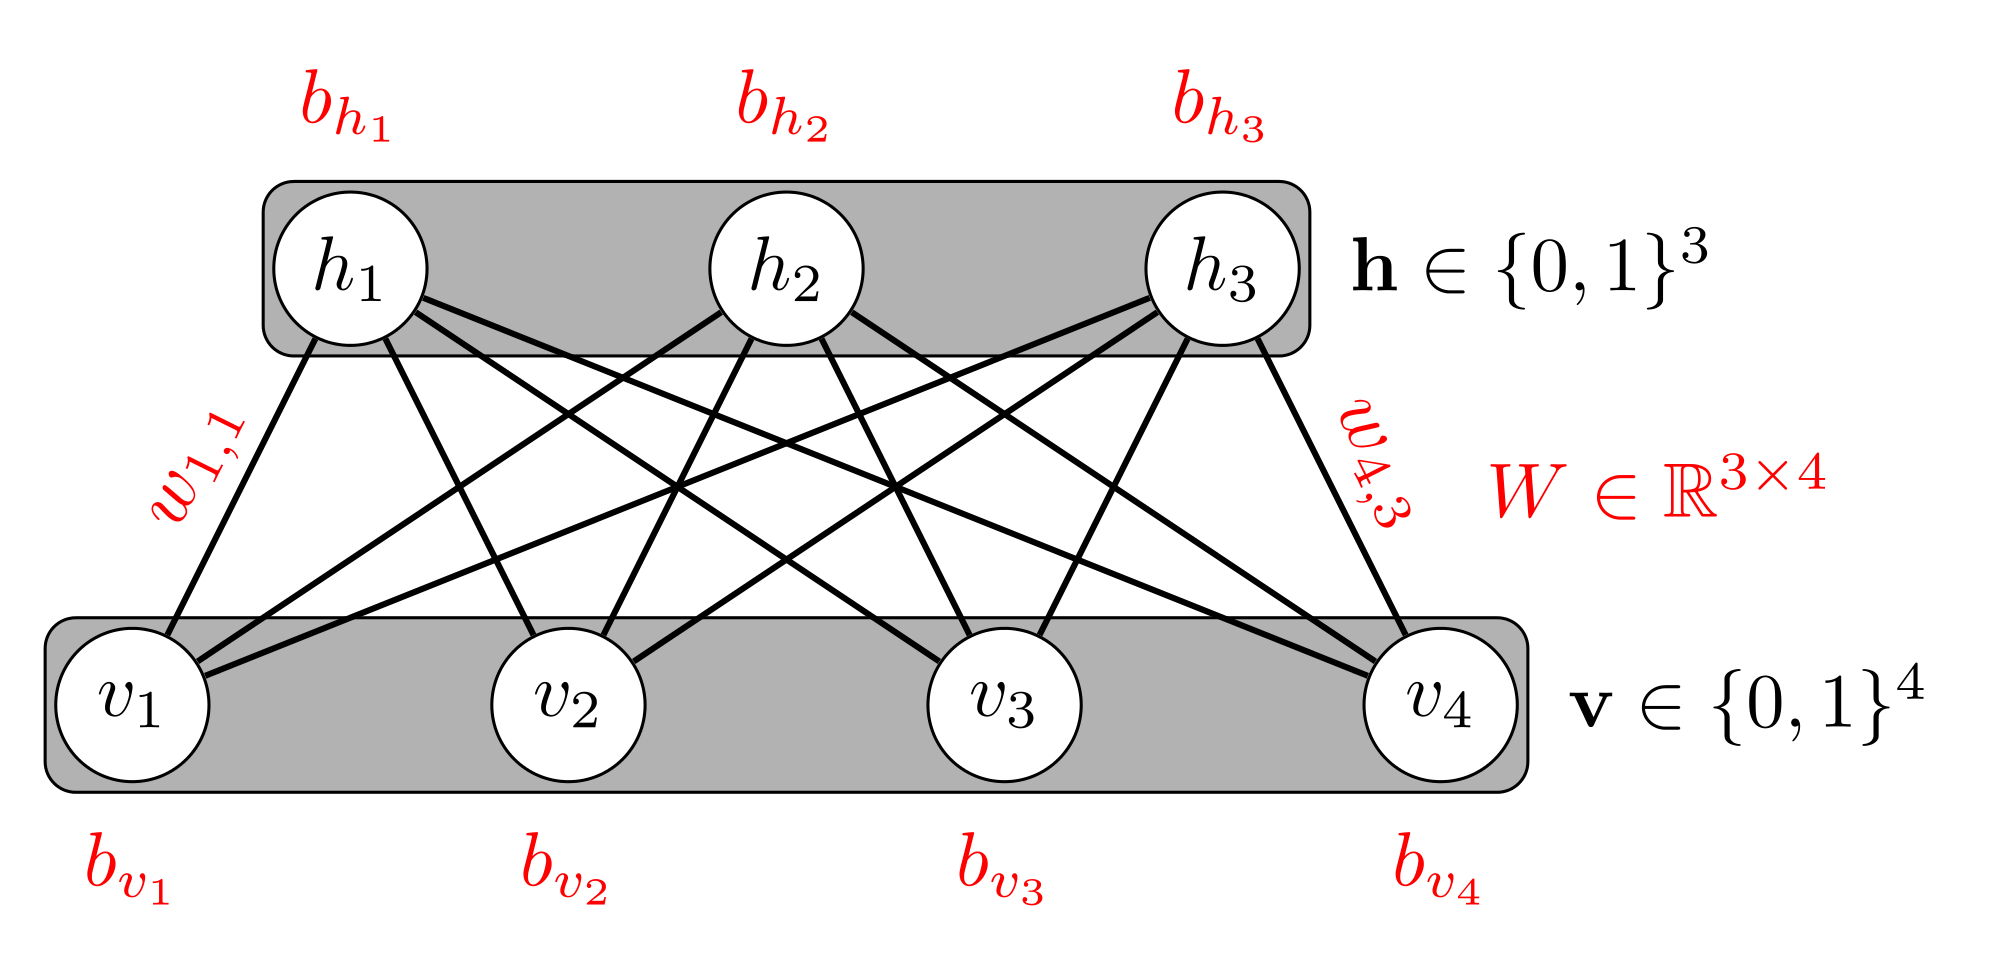
\includegraphics[width=0.45\textwidth]{figures/rbm.png}
    \caption{Restricted Boltzmann Machine.
        Figure courtesy of https://commons.wikimedia.org/wiki/File:Restricted-boltzmann-machine.svg}
    \label{Fig:RBMArchitecture}
\end{figure}


\subsection{Autoencoders}
An autoencoder neural network is an unsupervised model with typically one hidden layer that
tries to set the output layer to be equal to the input.
As shown in Figure~\ref{Fig:AEArchitecture}, we want the network to
learn a function $h_{W, b}(x) \approx x$.
However, to prevent the network from learning the meaningless identity function,
we need to place extra constraints on the network, giving birth to different
flavors of autoencoders.
In this project we consider one of the most popular types of autoencoder, sparse autoencoder.

\begin{figure}[h]
    \centering
    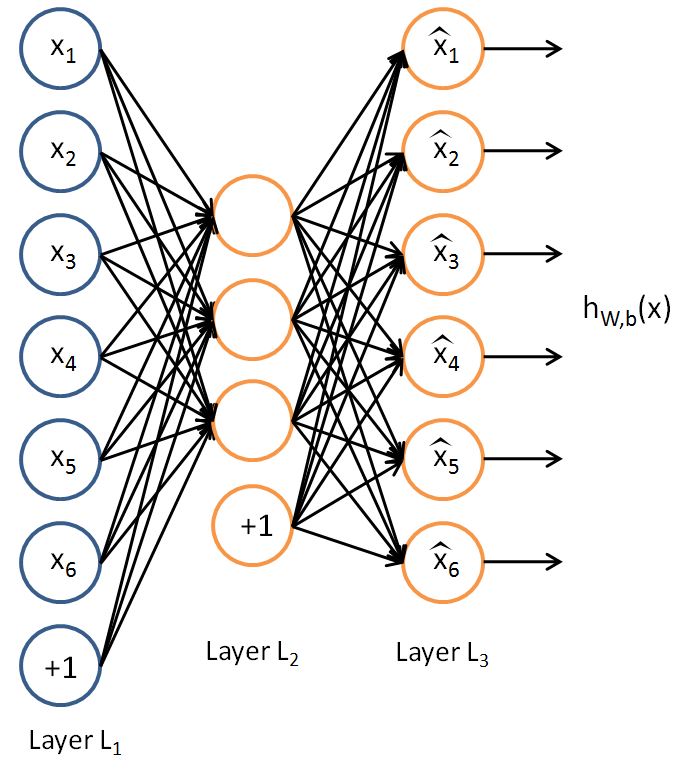
\includegraphics[width=0.45\textwidth]{figures/autoencoder.png}
    \caption{General Architecture of Autoencoders.
        Figure courtesy of~\cite{UFLDLAutoencoder}.}
    \label{Fig:AEArchitecture}
\end{figure}

\iffalse
The \textbf{denoising autoencoder} algorithm is proposed by~\cite{DenoiseAE} and illustrated in
Figure~\ref{Fig:dAEAlgorithm}.
To prevent learning identity function, an example $\mathbf{x}$ is first corrupted, either by
adding Gaussian noise or by random masking a fraction of items in $\mathbf{x}$ to zero.
The autoencoder then maps corrupted $\mathbf{\tilde{x}}$ to a hidden representation $\mathbf{y} = sigmoid(\mathbf{W}\tilde{\mathbf{x}} + \mathbf{b})$.
From $\mathbf{y}$ we reconstruct $\mathbf{z}=g_\theta'(\mathbf{y})$.
The training needs to learn the parameters $\theta$ and $\theta'$ so that
average reconstruction error is minimized over training set.
For binary input $\mathbf{x}$, usually cross entropy is adopted as $L_H(\mathbf{x}, \mathbf{z})$;
while mean squared error is used for real-valued $\mathbf{x}$.

Denoising autoencoder and sparse autoencoder, surprisingly, have different application domains.
Vincent et al.~\cite{DenoiseAE} have shown that stacked denoising autoencoder can be used to
initialize a deep neural network's weight parameter,
achieving similar and sometimes better performance than stacked RBM.
They also show that training stacked denoising autoencoder with MNIST dataset, it is able
to re-synthesize a variety of similarly good quality digits.
Raina et al.~\cite{SparseAE} have compared sparse encoding with principle component analysis
(PCA) and argue that transferring raw features with a well unsupervised trained
sparse autoencoder can be beneficial to supervised learning algorithms,
for example support vector machines (SVM).
\begin{figure}[h]
    \centering
    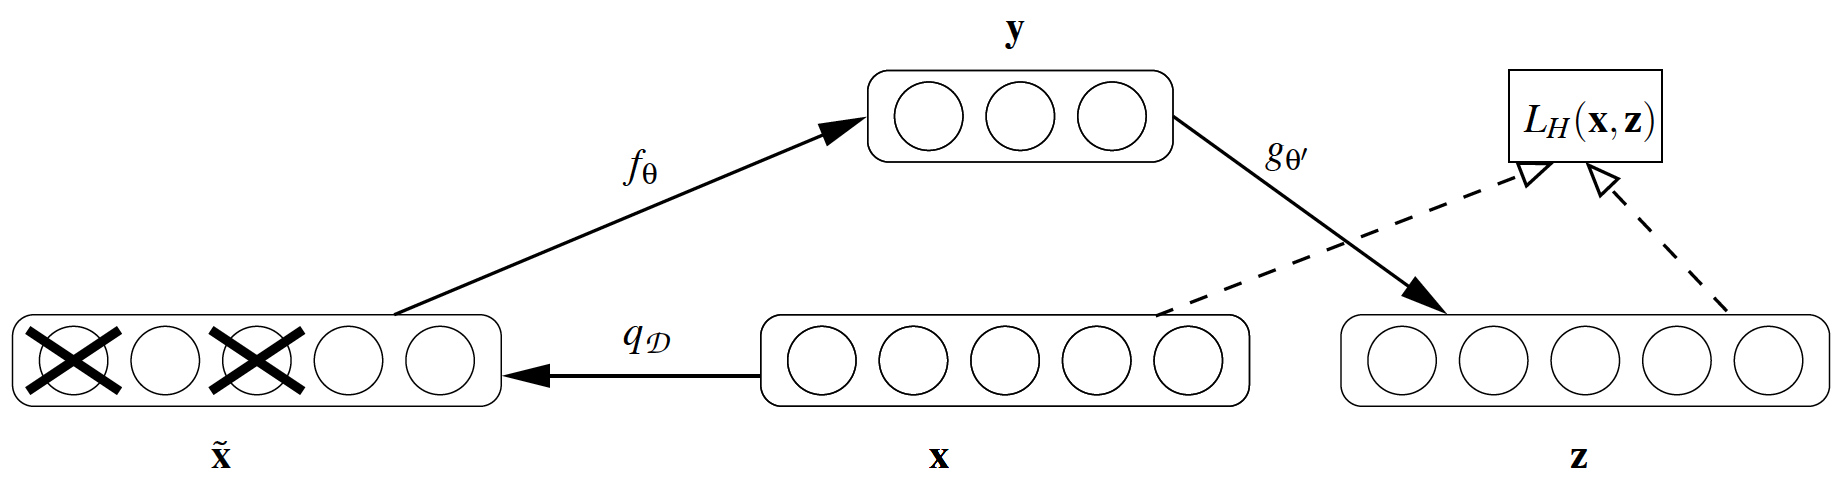
\includegraphics[width=0.45\textwidth]{figures/denoiseautoencoder.png}
        \caption{The denoising autoencoder algorithm.
        Input example $\mathbf{x}$ is randomly corrupted via $q_\mathcal{D}$ and then
        is mapped via encoder $f_\theta$ to $\mathbf{y}$.
        The decoder $g_\theta'$ attempts to reconstruct $\mathbf{x}$ and produces $\mathbf{z}$.
        Reconstruction error is measured by loss $L_H(\mathbf{x}, \mathbf{z})$, to be minimized
        during the training phase.
        Figure courtesy of~\cite{DenoiseAE}.}
    \label{Fig:dAEAlgorithm}
\end{figure}

\fi

The \textbf{sparse autoencoder} works by placing a sparsity constraint on the hidden units~\cite{SparseAE}.
First, we make the autoencoder's hidden layer size to be over-complete,
that is, of larger size comparing to the dimension of the input.
Let's denote the activation of hidden unit $j$ of layer 2 in Figure~\ref{Fig:AEArchitecture}
to be $a^2_j(\mathbf{x})$ given input example $\mathbf{x}$.
With that, we define the average activation of hidden unit $j$ over the $m$-size
training set
\begin{align}
    \hat{\rho}_j = \frac{1}{m} \sum_{i=1}^{m} a^2_j(\mathbf{x})
\end{align}
The sparsity constraint is enforcing, $\forall$ hidden unit $j$,
\begin{align}
    \hat{\rho}_j = \rho
\end{align}
where $\rho$ is a sparsity parameter that approximates zero (say 0.05).
This constraint can be vectorized over the hidden layer, say of size $n_2$,
with the KL divergence based penalty term
\begin{align}
    \sum_j^{n_2} KL(\rho || \hat{\rho}_j)
    = \sum_j^{n_2} [\rho \log \frac{\rho}{\hat{\rho}_j} + (1 - \rho) \log \frac{1-\rho}{1-\hat{\rho}_j} ]
\end{align}
The sparsity penalty term is integrated into the cost function by adding another hyper-parameter $\beta$
\begin{align}
    L(W, b) = \frac{1}{2}||h_{W,b}(\mathbf{x}) - \mathbf{x}||^2 +
    \beta \sum_j^{n_2} KL(\rho || \hat{\rho}_j)
\end{align}

Our implementation of the sparse autoencoder is different from the
self-taught learning approaches in~\cite{STL-NIDS, SparseAE},
which also adopting sparse autoencoder as the unsupervised feature learner.
In their work, the hidden features learnt by sparse autoencoders are used directly by
a classifier, for example, a softmax regressor or a SVM.
The functionality of autoencoder resembles a transformation of raw dataset
by approaches such as principle component analysis,
aiming to obtain a new feature space beneficial to general supervised learning algorithms.

Our way of utilizing autoencoder is to initialize the first layer weights of a MLP,
similar to how we use RBM.
The over-complete hidden layer size of the sparse autoencoder is 800;
the sparsity value $\rho$ is 0.05.
The autoencoder is trained with ADADELTA~\cite{ADADELTA} for 200 epochs and batch size 80.
We then create a separate MLP with same configuration as that in section~\ref{SubSec:MLP}
and initialize its first layer weights with the learnt weights of the autoencoder.
During finetuning the MLP, we used SGD optimizer with very small initial learning rate 0.004
and decaying 1e-6 over each update.
We denote this approach as SAE and report its performance in the later section.


\iffalse
\subsection{Generative Adversarial Nets}
As another generative model, Generative Adversarial Nets (GAN)\cite{GAN} adopts a novel training framework,
in which two models are trained simultaneously and adversarially.
The generative model $G(z;\theta_g)$ aims to capture the probability distribution of the available unlabelled dataset,
where its input is a noise variable $z$ following a prior distribution $p_z$.
The discriminative model $D(x;\theta_d)$ output the probability distribution that whether the its input source $S$ comes
from training dataset ($x\sim data$) or the generative model ($x \sim G(z)$):
\begin{align}
    D(X) = P(S|X)
\end{align}

Models $G$ and $D$ can be as simple as multilayer perceptrons,
or as complex as deep convolutional nets when the task domain is image.
The two models are trained in opposition to one another, with respect to the following log-likelihood function

\begin{align}
V(D, G) & = \mathbb{E}_{\bm{x}\sim data} [\log P(S=real|X=\bm{x})] + \mathbb{E}_{\bm{x}\sim G(\bm{z})} [\log P(S=fake|X=\bm{x})] \\
        & = \mathbb{E}[\log D(\bm{x})] + \mathbb{E}[\log (1 - D(G(\bm{z})))]
\end{align}

With $V(D, G)$ properly defined, the training procedure is a two-player minimax game.
First we maximize the log-likelihood that $D$ correctly recognize
both the training examples and the samples generated from $G$;
in the following phase, we train $G$ to generate samples that trick $D$ to make most mistakes.
This two-phase min-max optimization can be summarized as:
\begin{align}
    \min_G \max_D V(D, G)
\end{align}

Powerful though GAN is, large amount of efforts and care are needed during training.
One way to make the training stable and fast is to augment GAN with an auxiliary classifier so that
the training phase employs the labels available in the dataset~\cite{AC-GAN}.
In auxiliary classifier GAN (AC-GAN), the discriminator $D$ now gives both the probability
distribution over the sources (whether $\bm{x}$ is real or fake) and the probability distribution
over the class labels:
\begin{align}
    D(X) = P(S|X), P(C|X)
\end{align}
Accordingly, the log-likelihood function $V(D, G)$ is augmented with the log-likelihood of the correct class $L_C$:

\begin{align} 
    V(D, G) &= L_S + L_C \\
    L_S &= \mathbb{E}_{\bm{x} \sim data} [\log P(S=real|X=\bm{x})] + 
    \mathbb{E}_{\bm{x} \sim G(\bm{z})} [\log P(S=fake|X=\bm{x})] \\
    L_C &= \mathbb{E}_{\bm{x} \sim data}[\log P(C=c|X=\bm{x})] + 
    \mathbb{E}_{\bm{x} \sim G(\bm{z})} [\log P(C=c|X=\bm{x})]
\end{align}

The training procedure for AC-GAN is similar to GAN: we train $D$ to maximize $V(D, G)$;
while at the same time we train $G$ to minimize $L_S - L_C$.
Currently, we are interested in using GAN or AC-GAN to generate fake traffic.
In the future, we will also attempt the semi-supervised classification framework with AC-GAN.
\fi

\subsection{Wide and Deep Learning with Embeddings}
\label{SubSec:WD}
In the network intrusion dataset, categorical and integer features are extremely sparse.
For illustration reason, we plot the histogram of the ``dloss" integer feature in UNSW-NB15 dataset,
which denotes the number of destination packets retransmitted or dropped.
As shown in~\ref{Fig:DlossHist}, ``dloss"'s values range from 0 to 6000, while more than 97\%
of the occurred value is 0 but values from 1000 to 6000 do appear in the dataset.
For categorical feature ``proto", which tells one of the 133 protocol types the traffic record belongs to,
one-hot encoding it will make it become a 133-dimension vector with only one field being one.
Usually neural networks are not good at utilizing sparse large dimension input.

We tackle this problematic situation in two ways,
resulting in the combined model proposed in~\cite{WideDeepModel}.
The first solution is to embed the integer or categorical features.
Simply put, an embedding is a mapping from sparse discrete objects to a dense vector of real numbers.
It is widely used, also known as ``word2vec", in the natural language processing and machine translation tasks,
where embeddings are treated as points in vector space such that similarity between objects can be visually measured
by the Euclidean distance or angle between vectors.
In our case, embedding provide a solution to converting large-vocabulary-size categorical features
and sparse integer features to dense vectors of continuous values.
Deep neural network fed with embedding inputs can generalize better even with less feature engineering.
As stated in~\cite{WideDeepModel}, these input features to the deep neural nets are denoted as deep components,
consisted of continuous, one-hot encoded, and embedded features.

On the other hand, we leverage simple linear models with nonlinear feature transformations to deal with sparse inputs,
namely the wide components proposed in~\cite{WideDeepModel}.
The wide components consist of two parts: the basis and crossed features.
The basis features are raw input features that are either integer or categorical.
The crossed features are cross-product transformations of basis features:
\begin{align}
    \Phi_k (\bm{x} ) = \prod_{i=1}^{d} {x_i}^{c_{ki}}
\end{align}
where
\begin{align}
    c_{ki} = 
    \begin{cases}
        1, & \text{$i$-th feature $\in$ the transformation $\Phi_k$} \\
        0, & \text{otherwise}
    \end{cases}
\end{align}

\begin{align}
    \Phi_k (\mathbf{x} ) = \prod_{i=1}^{d} {x_i}^{c_{ki}}, \text{ where }
c_{ki} = 
\begin{cases}
    1, & \text{$i$-th feature $\in \Phi_k$} \\
    0, & \text{otherwise}
\end{cases}
\end{align}
The function of wide components, especially the cross-product transformations,
is memoization of the raw feature interactions.

In summary, the Wide and Deep model actually complements a deep neural network
with embedded low-dimension input vectors for good generalization;
Its linear sub-model, as shown in Figure~\ref{Fig:WideDeepModel}, is integrated with the deep neural network using a weighted sum of each model's output for good memorization.

The wide and deep learning model requires engineering the raw attributes in dataset into basis, crossed, continuous, and embedded components.
In our implementation, the basis features are all the raw symbolic and integer attributes.
Crossed features are built by a subset of combinations of the symbolic attributes in a dataset.
The raw symbolic and integer attributes are fed to the deep neural network as embedded components after conducting embedding.
The continuous components are straitforwardly the raw continuous attributes.
To compare with previous proposed models, we set the structure of the deep neural network in the wide and deep model to be
the same sizes as that of the baseline MLP, namely two hidden layers with size of [800 480].

\begin{figure}[h]
    \centering
    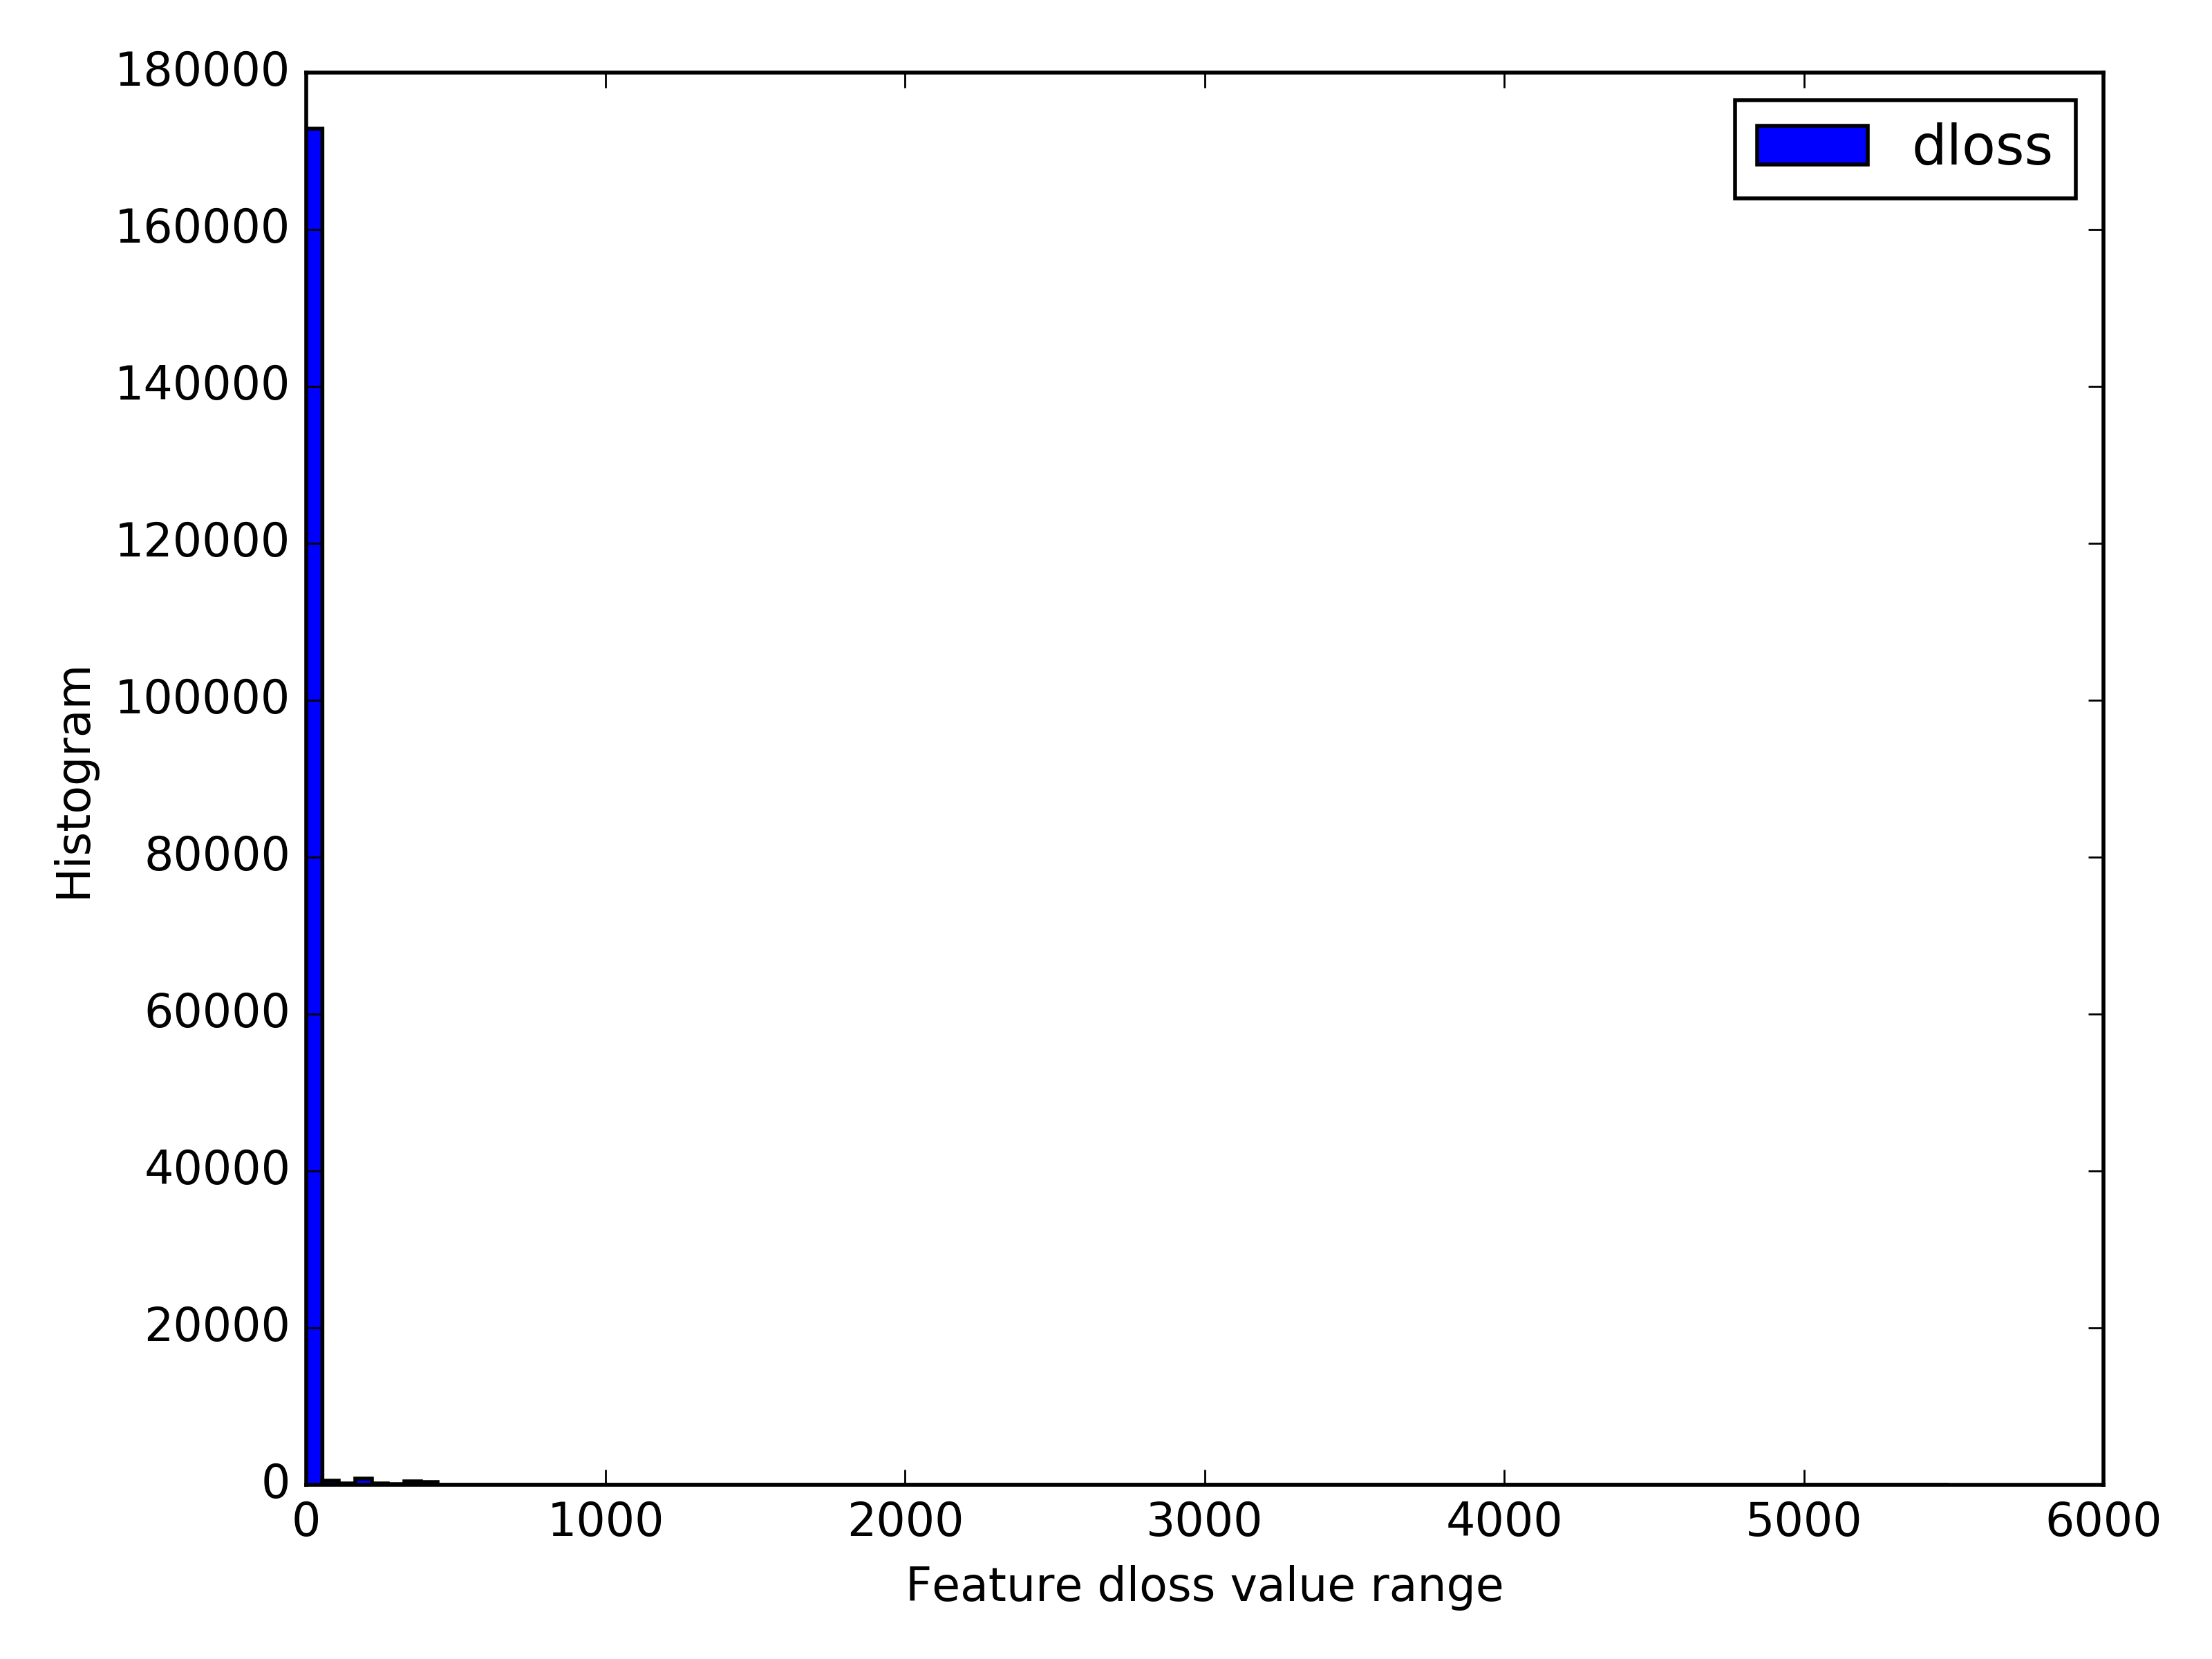
\includegraphics[width=0.45\textwidth]{figures/dloss_hist.png}
    \caption{Histogram of the Feature ``dloss" from UNSW-NB15 Dataset.}
    \label{Fig:DlossHist}
\end{figure}

\begin{figure*}[h]
    \centering
    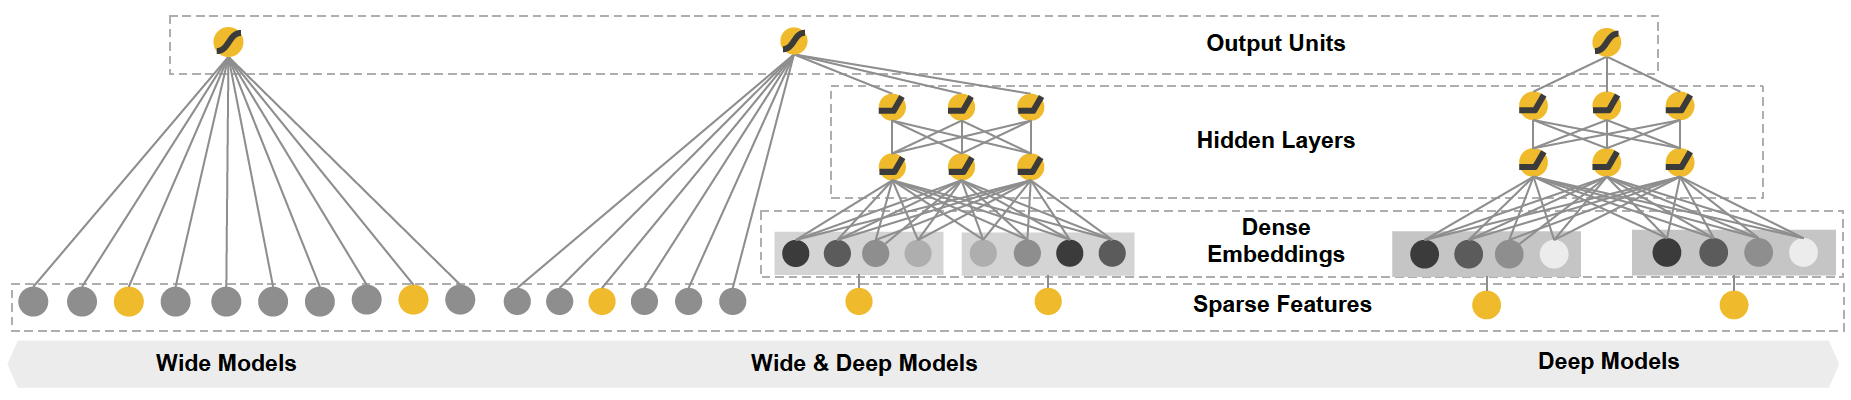
\includegraphics[width=0.98\textwidth]{figures/WideDeepModel.png}
    \caption{Anatomy of Wide and Deep Model}
    \label{Fig:WideDeepModel}
\end{figure*}

\section{Experimental Evaluation}

We evaluate all the models developed in NetLearner on the 5-class NSL-KDD task and the 2-class UNSW-NB15 task using the following metrics.
\begin{itemize}
    \item \textbf{Accuracy} is the percentage of correctly classified connections
        over the total number of connections in the dataset:
        \begin{align}
            A = \frac{\text{Correct Predictions}}{\text{Number of Records}}
        \end{align} 
        Accuracy is not suitable for evaluating biased datasets where the number
        of records of one class is extremely larger than the number of
        records of another class.
        In the NSL-KDD dataset, the number of available U2R records (i.e., 67)
        is two orders of magnitude less than the number of records in other classes
        (i.e., 9711, 7458, 2887 and 2121).
        Therefore, we also consider the precision and recall.
    \item \textbf{Precision} is the percentage of the correctly classified positives over
        the total number of positives predicted by the classifier.
                \begin{align}
                    P = \frac{\text{True Positives}}{\text{True Positives} + \text{False Positives}}
                \end{align}
    \item \textbf{Recall} is the percentage of the correctly classified positives over
        the total number of relevant elements.
                \begin{align}
                    R = \frac{\text{True Positives}}{\text{True Positives} + \text{False Negatives}}
                \end{align}
\end{itemize}
%The weight for each class is determined by its proportion in the test dataset,
%namely [0.431, 0.107, 0.339, 0.018, 0.105] for class [Normal, Probe, DoS, U2R, R2L] respectively.
%Besides, we also calculate the confusion matrices of the classification results when applying
%different approaches on both task's test datasets.
%In a confusion matrix table, the $i$th row represents the instances of class $i$,
%while the $j$th column represents the instances predicted by the classifier as class $j$.
%It is called confusion matrix because it is useful for visualizing how a classifier
%is confusing one class with other classes.
%Due to page space limit, here we only present the most straightforward
%and relatively more important metric accuracy.
%Statistics regarding precision, recall and confusion matrices can be found
%in our detailed technical report~\cite{OurWonReport} and our codebase~\cite{NetLearner}.

We train an radial basis function kernel support vector machine (SVM)% using the approach in ~\cite{ScikitLearnSVM},
and report its accuracy with the multilayer perceptron (MLP) model,
the restricted Boltzmann machine fine-tuned neural network (RBM),
the sparse autoencoder fine-tuned neural network (SAE),
and the wide linear classifier and deep neural network combined model (WnD).

It is critical to search the optimal hyper-parameters that fit the problem domain and model before training machine learning models. We first manually set all the hyper-parameters, including the number of layers, number of neurons in each layer, learning rate, and batch size, to be identical across all the models.
We then use 5-fold cross-validation on the training datasets to determine the optimal training time $T$
for each model.
Finally, we train the model for $T$ epochs and report the metrics on the testing dataset,
which is not touched during the training phase.
Determining the training time (model complexity) by cross-validation with fixed common hyper-parameters
ensures that the deep learning models are neither overfitting nor underfitting.
As illustration purpose, we plot the MLP's 5-fold cross validation loss in Figure~\ref{Fig:LossHistory},
from which we can see that validation loss converges to $\approx$0.02 after 120 epochs, even though training loss is still decreasing.

The accuracies of each classifier are shown in Figure~\ref{Fig:CompAccuracyNSL} for the NSL-KDD task and Figure~\ref{Fig:CompAccuracyUNSW} for the UNSW-NB15 task.
In the 2-class UNSW-NB15 dataset,
the volumes of normal and attacking traffic are nearly balanced (i.e., 37,000 normal v.s. 45,332 attacking records).
Therefore, we only report the precision and recall for the attacking traffics in Figure~\ref{Fig:CompAccuracyUNSW}.
For the 5-class NSL-KDD task, we adopt the approach in~\cite{STL-NIDS}
to calculate the weighted precisions and recalls, and plot them together with accuracy in Figure~\ref{Fig:CompAccuracyNSL}.
The per-class precisions and recalls are also listed in Table~\ref{Tab:PrecisionRecall}.

For the NSL-KDD task, all classifiers achieve high training accuracy (no less than 99\%).
However, all classifiers show a gap between training accuracy and testing accuracy (as low as 78.4\%).
As the representative of the classic machine learning approach, SVM achieves a 78.5\% accuracy
comparable to the deep learning models.
Note that our SAE model achieves the same accuracy performance to~\cite{STL-NIDS}, which is the best among all the considered models (79.2\%).
RBM, SAE, and WnD all outperform MLP for two different reasons.
RBM and SAE provide their underlying MLP with better initial weights in the first layer
than randomly generated numbers.
WnD has a slightly higher accuracy because of the extra linear model.
Table~\ref{Tab:PrecisionRecall} shows two remarkable facts.
SVM performs better at Probe attacks (93\% precision and 82\% recall)
than all the neural networks ($\approx$ 85\% precision and $\leq$ 70\% recall),
However, it suffers hugely on U2R attacks ($\approx$ 6\% precision and recall).
On the other hand, the neural networks (MLP, RBM, SAE and WnD) miss many U2R attacks ($\leq$ 6\% recall), but they have much higher reliability in identifying these attacking traffic ($\approx$ 60\% precision).

For the UNSW-NB15 task, the average accuracies of RBM, SAE and WnD are
all higher than MLP for the same reason mentioned in the NSL-KDD task.
We notice WnD has significantly improved MLP's performance by around 5\%.
Different from the NSL-KDD task, the training accuracies of all the approaches are mediocre (up to 94.4\%) in contrast to the NSL-KDD case where the training accuracy of every model is more than 99\%.
The harder UNSW-NB15 training dataset is one primary reason that the testing accuracies of the UNSW-NB15 task
are higher than that of the NSL-KDD task, since classifiers only have access to the training dataset.
Therefore, even though SVM has an equivalent training accuracy to the neural networks (93\% v.s. 94\%),
its testing accuracy falls far behind by 5\% (comparing to MLP) to 9\% (comparing to WnD),
showing the superior generalization capability of the deep neural network models.
The detection alarms are mostly correct for every classifier,
due to the high recall values $\geq$ 97\%, and the deep learning models have better precision ($\geq$ 81\%) than SVM (75\%).

\begin{figure}[h]
    \centering
    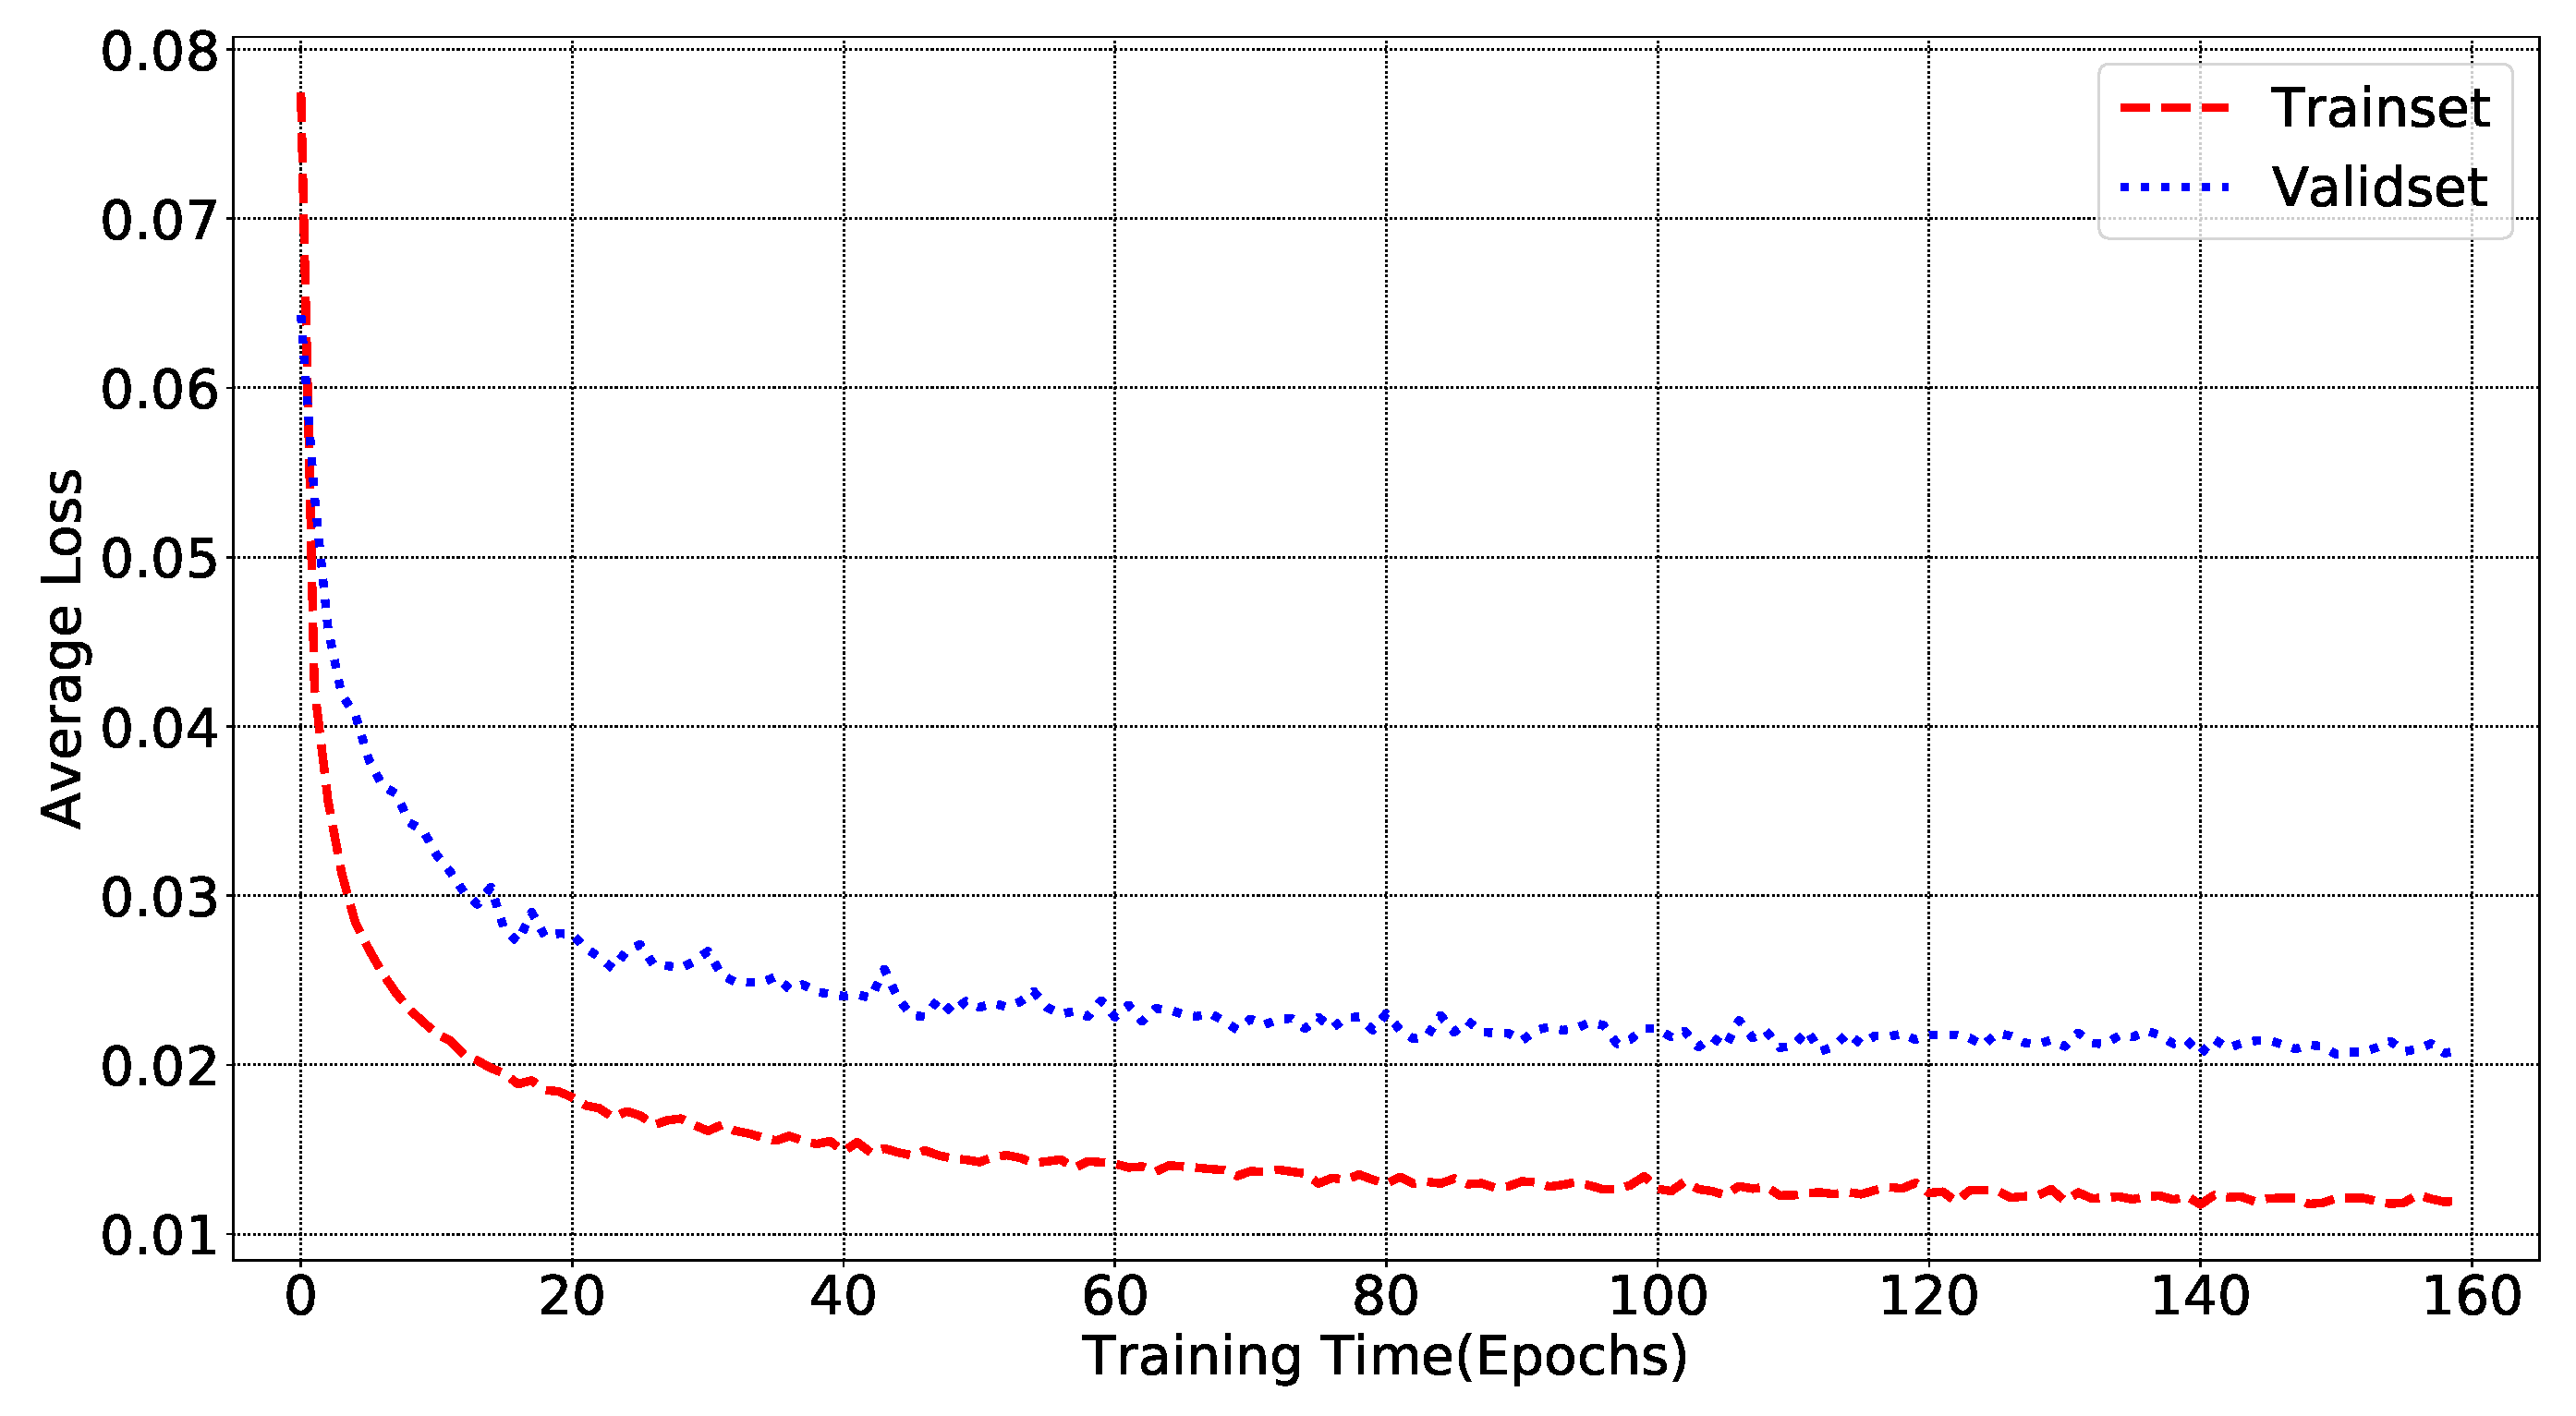
\includegraphics[width=0.48\textwidth]{figures/history.pdf}
    \caption{History of MLP's Average Loss During Cross Validation}
    \label{Fig:LossHistory}
\end{figure}

\begin{figure}[h]
    \centering
    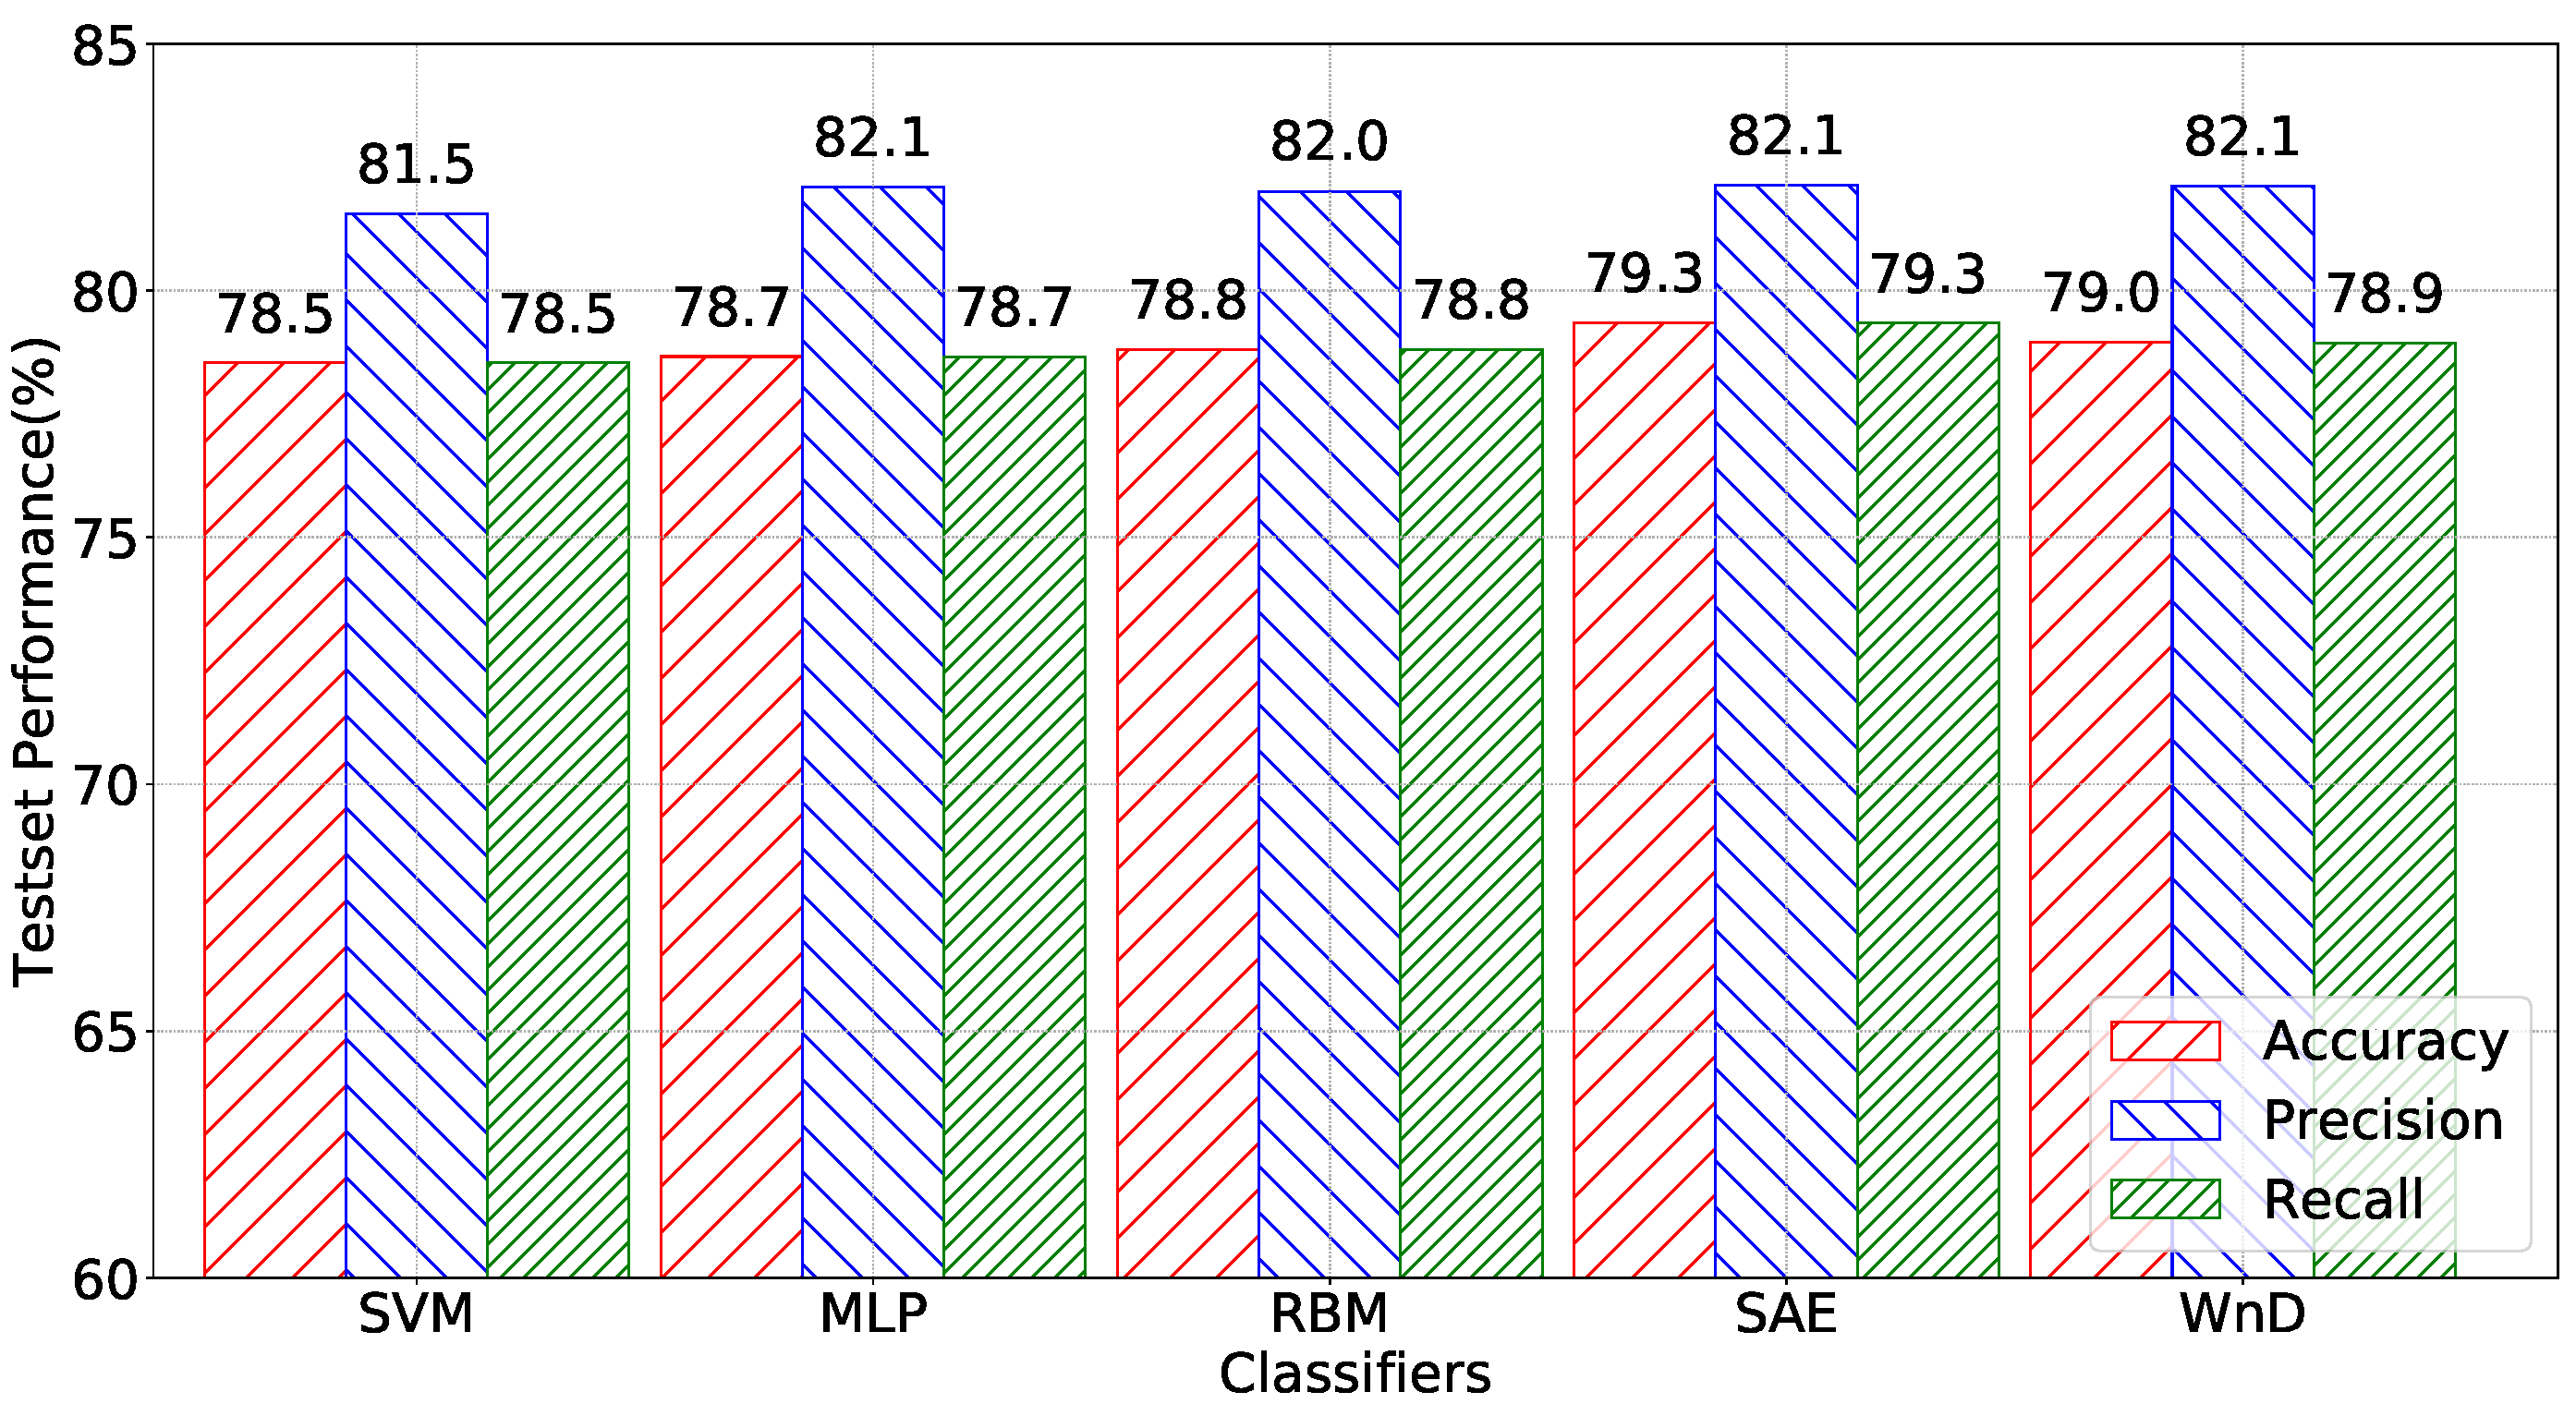
\includegraphics[width=0.48\textwidth]{figures/comp_accuracy_nsl.pdf}
    \caption{Metrics Comparison, NSL-KDD Task}
    \label{Fig:CompAccuracyNSL}
\end{figure}

\begin{figure}[h]
    \centering
    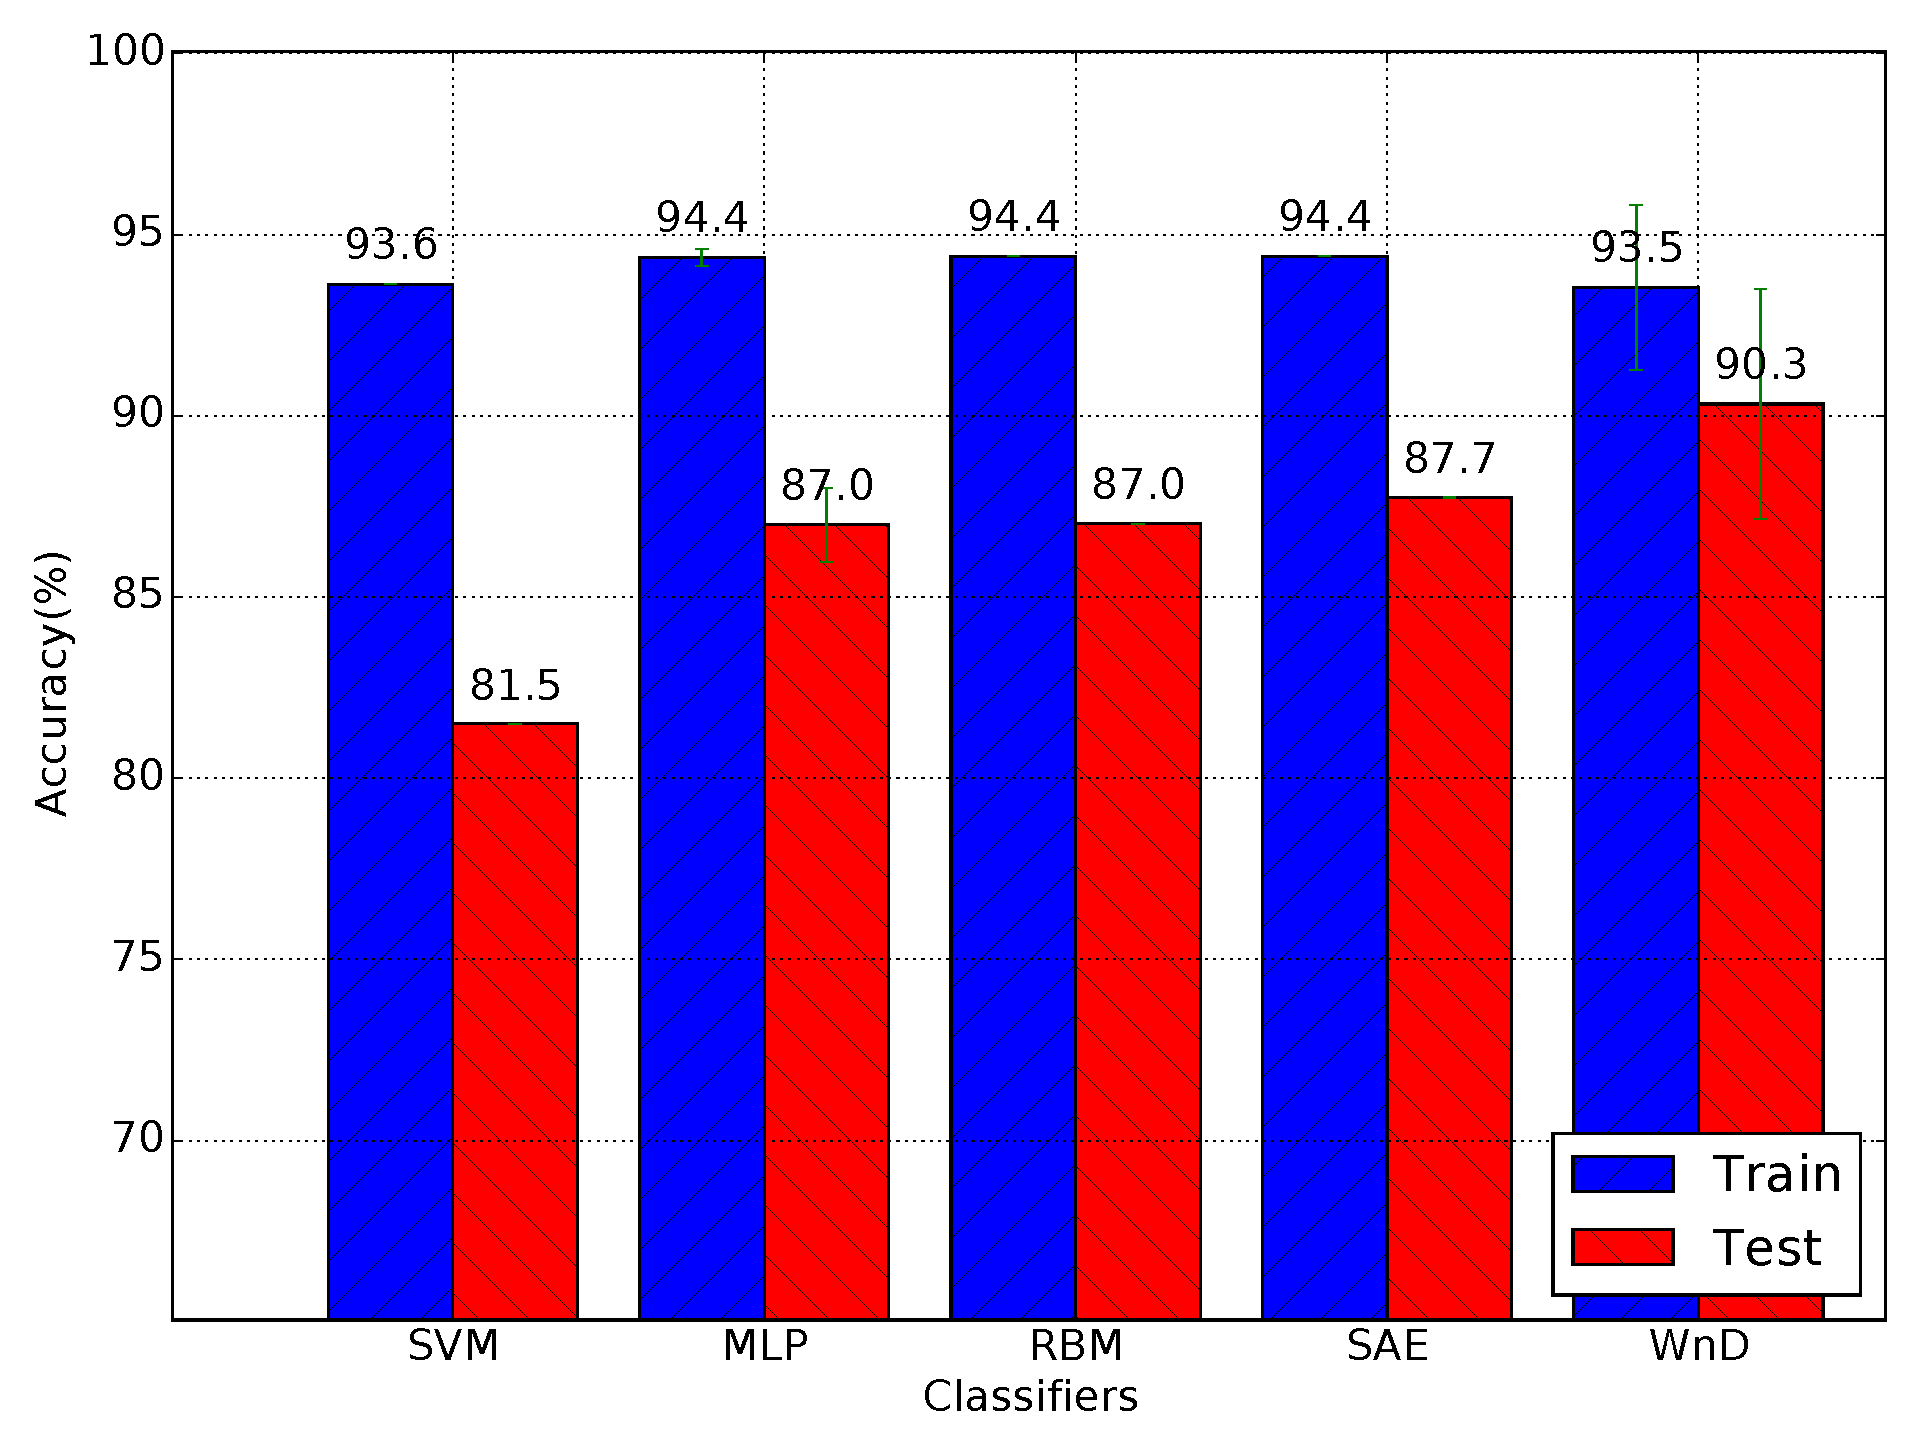
\includegraphics[width=0.48\textwidth]{figures/comp_accuracy_unsw.pdf}
    \caption{Metrics Comparison, UNSW-NB15 Task}
    \label{Fig:CompAccuracyUNSW}
\end{figure}

\begin{table}[]
    \centering
    \caption{Per-class Precision/Recall on the NSL-KDD Task}
    \label{Tab:PrecisionRecall}
    \begin{tabular}{c|c|ccccc}
        \hline
        \hline
                             &            & \multicolumn{5}{c}{Traffic Class} \\
        \cline{3-7}
                             &            & Normal & DoS   & Probe & U2R   & R2L \\
        \hline
        \multirow{2}{*}{SVM} & Precision  & 72.82  & 75.27 & 93.85 &  6.32 & 96.65 \\
        \cline{2-2}
                             & Recall     & 96.18  & 72.16 & 82.16 &  6.06 & 13.34 \\
        \hline
        \multirow{2}{*}{MLP} & Precision  & 69.18  & 95.49 & 85.58 & 59.52 & 92.01 \\
        \cline{2-2}
                             & Recall     & 96.66  & 82.31 & 69.28 &  6.31 & 15.03 \\
        \hline
        \multirow{2}{*}{RBM} & Precision  & 69.41  & 95.41 & 85.23 & 41.51 & 93.86 \\
        \cline{2-2}
                             & Recall     & 96.81  & 83.89 & 64.74 &  5.56 & 15.48 \\
        \hline
        \multirow{2}{*}{SAE} & Precision  & 70.20  & 95.63 & 84.70 & 65.00 & 87.76 \\
        \cline{2-2}
                             & Recall     & 96.92  & 83.34 & 70.56 &  3.28 & 16.29 \\
        \hline
        \multirow{2}{*}{WnD} & Precision  & 70.08  & 95.59 & 84.02 & 60.34 & 91.57 \\
        \cline{2-2}
                             & Recall     & 96.88  & 83.64 & 67.84 &  4.53 & 15.34 \\
        \hline
    \end{tabular}
\end{table}


\section{Conclusion}
We study cutting-edge deep learning models to the design of network intrusion detection systems.
%First, we briefly discuss general deep learning methodology and its potential implication on the network intrusion detection problem.
%Then we describe a set of promising deep learning models in concisely mathematical languages.
With the help of our open-source Tensorflow-based deep learning library NetLearner, we perform a comparative evaluation of those models on two network intrusion detection tasks using the NSL-KDD and UNSW-NB15 datasets. Preliminary experimental results show that for the NSL-KDD task, sparse autoencoder achieves accuracy similar to the existing machine learning solutions; for the UNSW-NB15 dataset, deep neural network models with greater generalization capability achieve better accuracy than SVM based solutions.
\section*{Acknowledgment}
The authors are grateful to the support by the Air Force Office of Scientific Research under Grant YIP FA9550-17-1-0240 and a cooperative agreement between IIT and National Security Research Institute (NSRI) of Korea.

\bibliographystyle{IEEEtran}
\bibliography{IEEEabrv,ref}

\end{document}

